% Sistema ortonormal y otro inclinado, con un vector (libro fig. 5.3)
\documentclass[border=5pt]{standalone}
\usepackage{tikz}
\usetikzlibrary{arrows.meta, calc}
\begin{document}
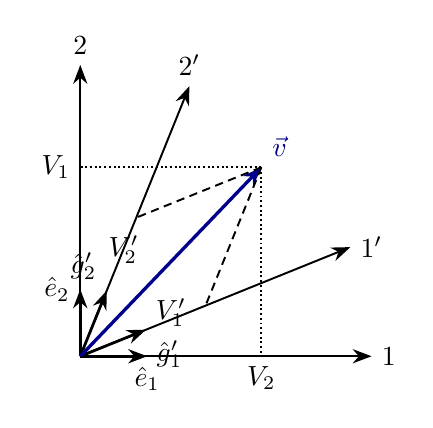
\begin{tikzpicture}[>={Stealth[length=2.4mm]}, line width=0.7pt]
  \coordinate (O) at (0,0);
  \coordinate (V) at (2.3,2.4);
  % ejes ortonormales
  \draw[->] (O)--(3.7,0) node[right]{$1$};
  \draw[->] (O)--(0,3.7) node[above]{$2$};
  % ejes inclinados
  \draw[->] (O)--(22:3.7) node[right]{$1'$};
  \draw[->] (O)--(68:3.7) node[above]{$2'$};
  % vectores base unitarios
  \draw[->, line width=1pt] (O)--(0.85,0) node[below]{$\hat e_1$};
  \draw[->, line width=1pt] (O)--(0,0.85) node[left]{$\hat e_2$};
  \draw[->, line width=1pt] (O)--(22:0.9) node[below right]{$\hat g'_1$};
  \draw[->, line width=1pt] (O)--(68:0.9) node[above left]{$\hat g'_2$};
  % vector v
  \draw[->, line width=1.2pt, blue!55!black] (O)--(V) node[above right]{$\vec v$};
  % componentes ortonormales (proyección perpendicular, punteado)
  \draw[densely dotted] (V)--(2.3,0); \node[below] at (2.3,0){$V_2$};
  \draw[densely dotted] (V)--(0,2.4); \node[left] at (0,2.4){\,$V_1$};
  % componentes inclinadas (proyección paralela, discontinuo)
  \draw[densely dashed] (V)--(1.59,0.64);
  \draw[densely dashed] (V)--(0.71,1.76);
  \node at (1.15,0.55){$V'_1$};
  \node at (0.55,1.35){$V'_2$};
\end{tikzpicture}
\end{document}
